\chapter{Definitions}

Since the main concern of this thesis is coloring of the graphs mentioned in the preface, it is useful to define all the necessary concepts we will be working with.

\section{Basic definitions and assumptions}

Here we state mathematical definitions, that should not be surprising in any way. Also, we state some assumption we will make, which will then hold for the rest of this thesis.

\begin{definition}
    An \textit{undirected graph} $G$ is an ordered pair $G=(V,E)$ where $V$ is a set of vertices of the graph and $E \subseteq \binom{V}{2}$ is the set of its edges. 
\end{definition}

\begin{assumption}
    For any graph $G=(V,E)$ we will assume $V \cap E = \emptyset$ 
\end{assumption}

\begin{definition}
    A \textit{partial function} is a function $f:X \rightarrow Y$ s.t. $\forall x \in X$ we have $f(x) \in Y$ or $f(x)$ is undefined.
\end{definition}

\section{General coloring}

As we will be working with many different colorings, to avoid repetition, we will define the notion of an abstract coloring which all the concrete colorings will share.

\begin{definition}
    For $k \in \mathbb{N}$ and a graph $G=(V,E)$ \textit{coloring} of $G$ is a partial function $c: V \cup E \rightarrow \{1,\ldots,k\}$ with a coloring rule $R$ that restricts, which elements of the graph cannot share the same color.
\end{definition}

In other words, coloring is an assignment of numbers to vertices, edges or both s.t. based on the coloring rule, certain vertices or edges cannot share the same color. The coloring rule is usually independent on the choice of graph.

\begin{definition}
    Let the set of all colorings sharing the same coloring rule $R$ be called a \textit{family of colorings}
\end{definition}

\begin{definition}
    For a graph $G=(V,E)$ and a family of colorings $F$, if there exists a coloring $c \in F$ s.t. $c: V \cup E \rightarrow \{1,\ldots,k\}$ for some $k \in \mathbb{N}$ then we say that $G$ is \textit{k-colorable}
\end{definition}

\begin{definition}
    For a graph $G=(V,E)$ and a family of colorings $F$, let \textit{chromatic number} $\chi ^F (G)$ be the minimum $k \in \mathbb{N}$ s.t. $G$ is k-colorable.
\end{definition}

\section{Concrete colorings}

\subsection{Vertex coloring}

\begin{definition}
    A \textit{vertex coloring} of a graph $G=(V,E)$ is a coloring $c : V \rightarrow \mathbb{N}$ belonging to family of colorings with the following coloring rule:
    \begin{equation}\label{eqn:vtx_rule}
        \forall u,v \in V, \quad \text{if } \{u,v\} \in E, \text{ then } c(u) \neq c(v). 
        \tag{$R_V$}
    \end{equation}
    We will denote this family of colorings by $F_V$.
\end{definition}

In other words, vertex coloring is an assignment of colors to each vertex s.t. no two vertices connected by an edge share the same color.

\begin{figure}[H]
    \centering
    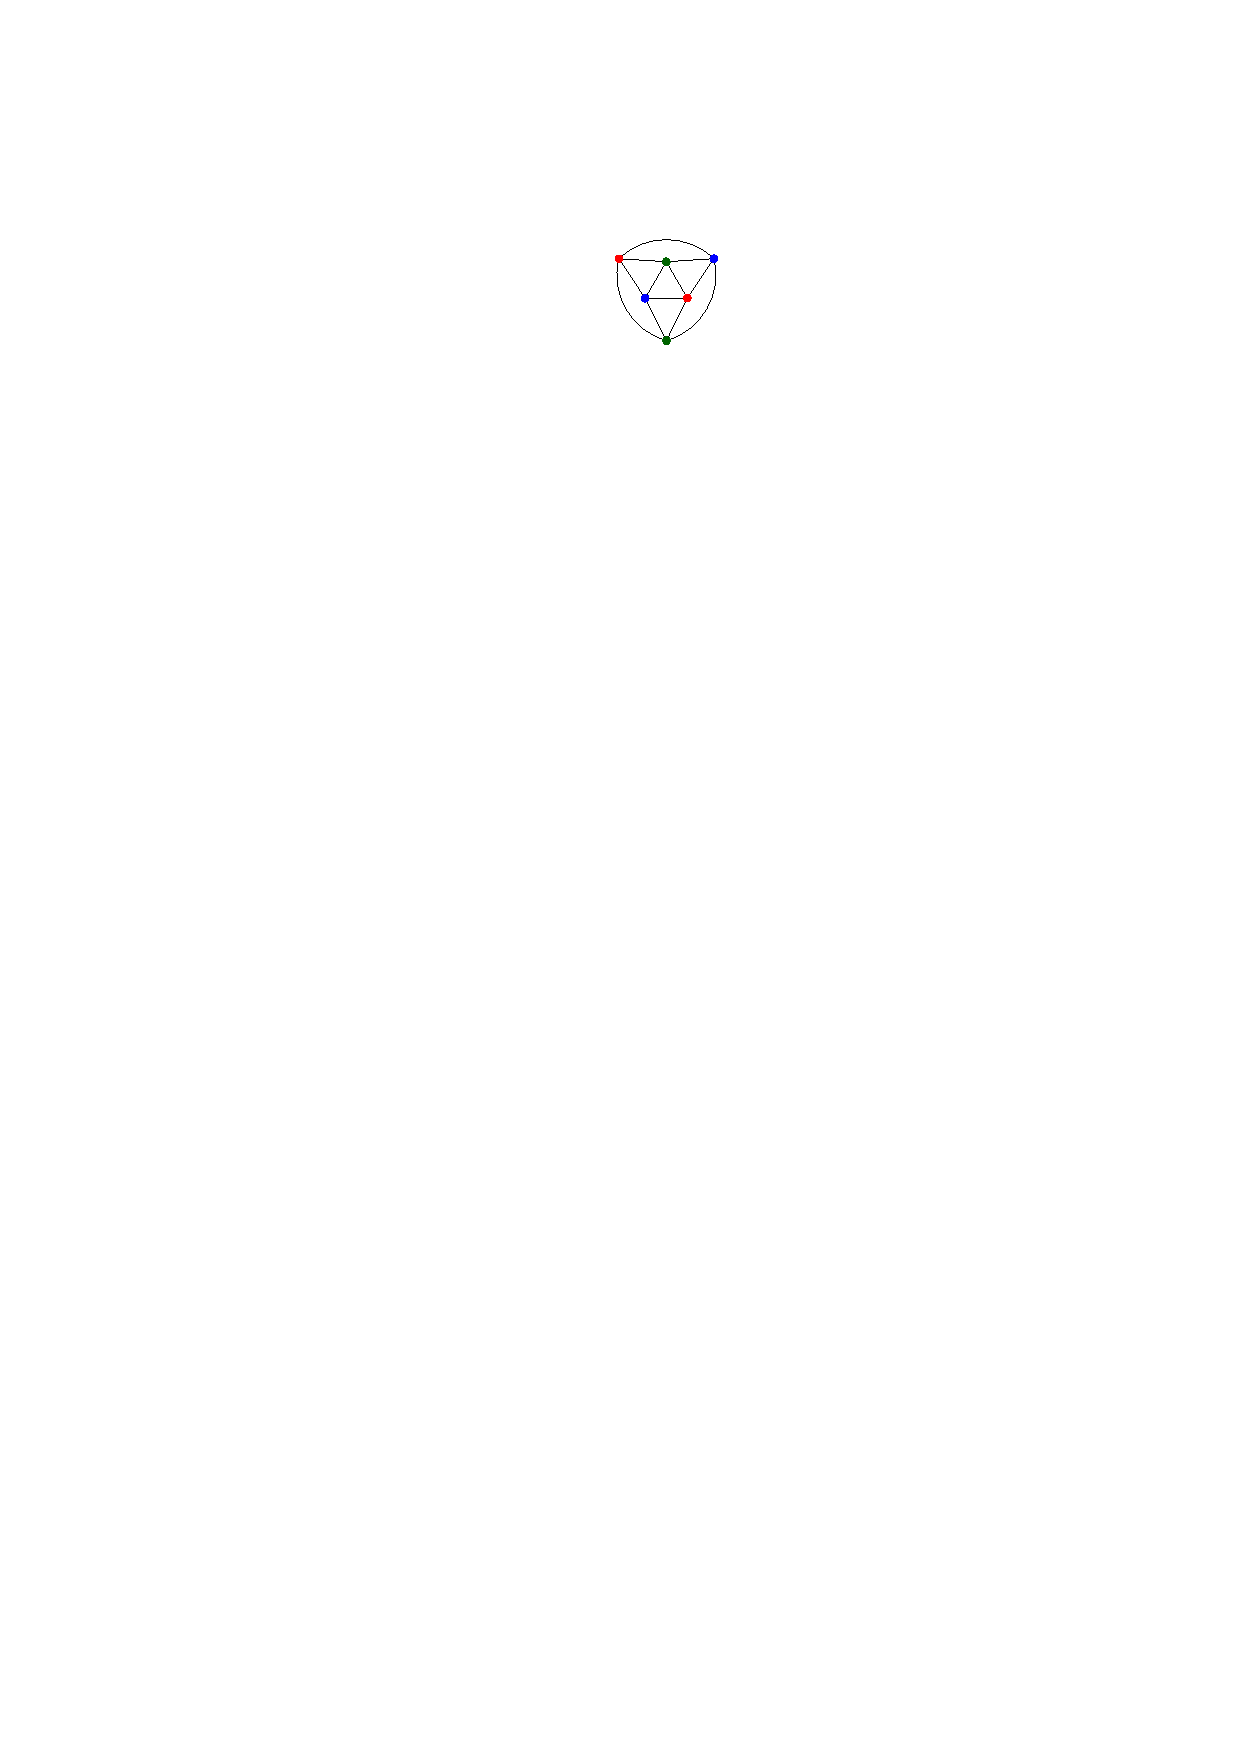
\includegraphics[width=0.2\textwidth]{../Resources/Figs/octahedral_vtx_colr.pdf}
    \caption{Vertex coloring of octahedral graph}
    \label{fig:octahedral_vtx_coloring}
\end{figure}

The graph in figure~\ref{fig:octahedral_vtx_coloring} has vertex chromatic number 3.

\subsection{Edge coloring}

\begin{definition}
    An \textit{edge coloring} of a graph $G=(V,E)$ is a coloring $c: E \rightarrow \mathbb{N}$ belonging to family of colorings for which the coloring rule is: 
    \begin{equation}\label{eqn:edge_rule}
     \forall e,f \in E, \quad \text{ whenever } e \cap f \neq \emptyset \text{ then } c(e) \neq c(f) \tag{$R_E$}
    \end{equation}
    We will denote this family of colorings by $F_E$.
   
\end{definition}

What the definition above says is, that whenever two edges share an endpoint, they cannot share the same color. 

\begin{figure}[H]
    \centering
    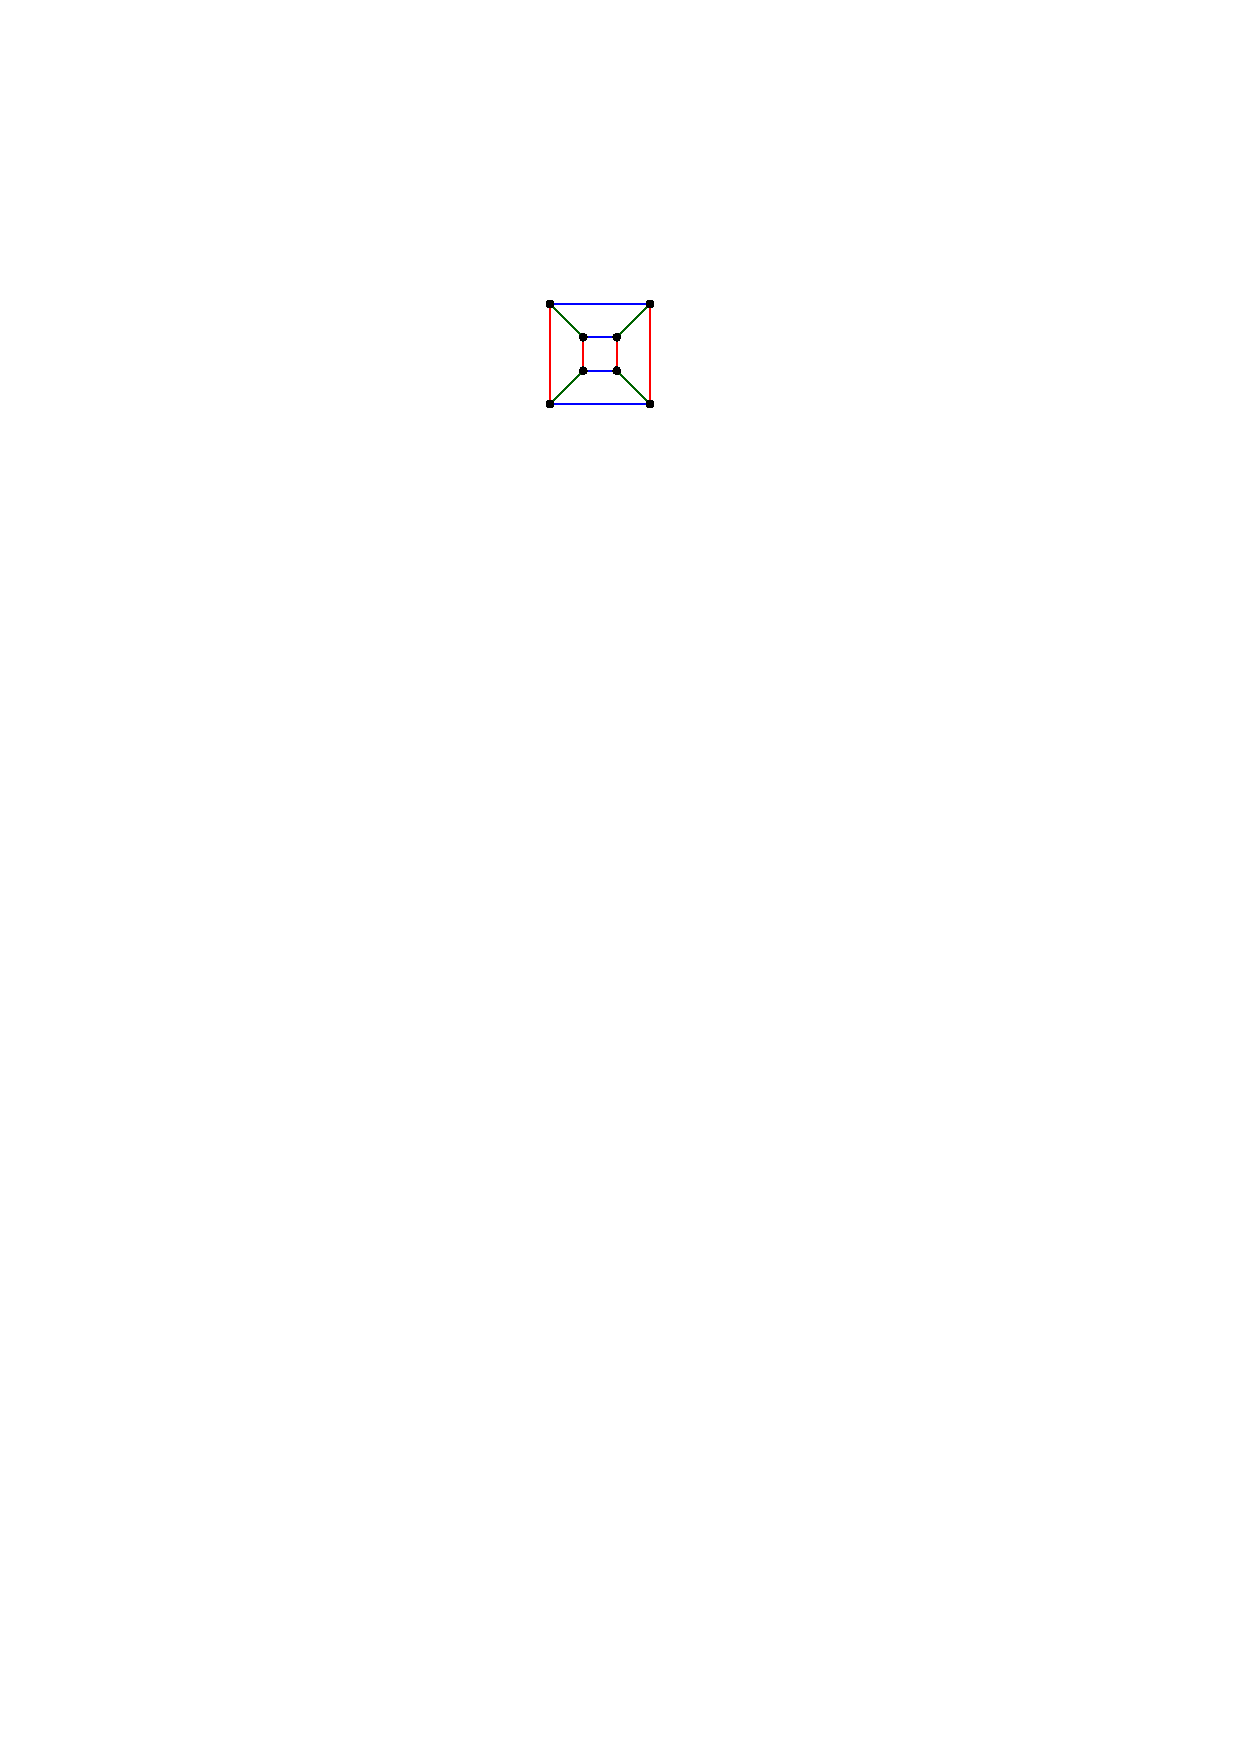
\includegraphics[width=0.2\textwidth]{../Resources/Figs/cubical_edg_colr.pdf}
    \caption{Edge coloring of cubical graph}
    \label{fig:cubical_edge_coloring}
\end{figure}

\subsection{Computed vertex and edge chromatic numbers}

The vertex and edge chromatic numbers can be computed in little time using \textit{SageMath} software. The following two tables provide overview of vertex chromatic numbers $\chi(G)$ and edge chromatic numbers $\chi^{'}(G)$ for Platonic and Archimedean solids.

\begin{center}
\begin{tabular}{|l|c|c|}
\hline
Platonic & $\chi(G)$ & $\chi^{'}(G)$ \\
\hline\hline
cube & 2 & 3 \\
\hline
dodecahedron & 3 & 3 \\
\hline
icosahedron & 4 & 5 \\
\hline
octahedron & 3 & 4 \\
\hline
tetrahedron & 4 & 3 \\
\hline
\end{tabular}
\end{center}

\begin{center}
\begin{tabular}{|l|c|c|}
\hline
Archimedean & $\chi(G)$ & $\chi^{'}(G)$ \\
\hline\hline
cuboctahedron & 3 & 4 \\
\hline
icosidodecahedron & 3 & 4 \\
\hline
rhombicosidodecahedron & 3 & 4 \\
\hline
rhombicuboctahedron & 3 & 4 \\
\hline
snub cube & 3 & 5 \\
\hline
snub dodecahedron & 4 & 5 \\
\hline
truncated cube & 3 & 3 \\
\hline
truncated cuboctahedron & 2 & 3 \\
\hline
truncated dodecahedron & 3 & 3 \\
\hline
truncated icosahedron & 3 & 3 \\
\hline
truncated icosidodecahedron & 2 & 3 \\
\hline
truncated octahedron & 2 & 3 \\
\hline
truncated tetrahedron & 3 & 3 \\
\hline
\end{tabular}
\end{center}


\subsection{Total coloring}

\begin{definition}
    A \textit{total coloring} of graph $G=(V,E)$ is a coloring $c: V \cup E \rightarrow \mathbb{N}$ from family of colorings sharing both coloring rules \ref{eqn:vtx_rule} and \ref{eqn:edge_rule} and the following additional rule: 
    \begin{equation}\label{eqn:tot_rule}
    \forall v \in V,  \forall e \in E, \text{ if } \{v\} \cap e \neq \emptyset \text{ then } c(v) \neq c(e) \tag{$R_T$}
    \end{equation}
    We will call this family $F_T$.
\end{definition}

\begin{figure}[H]
    \centering
    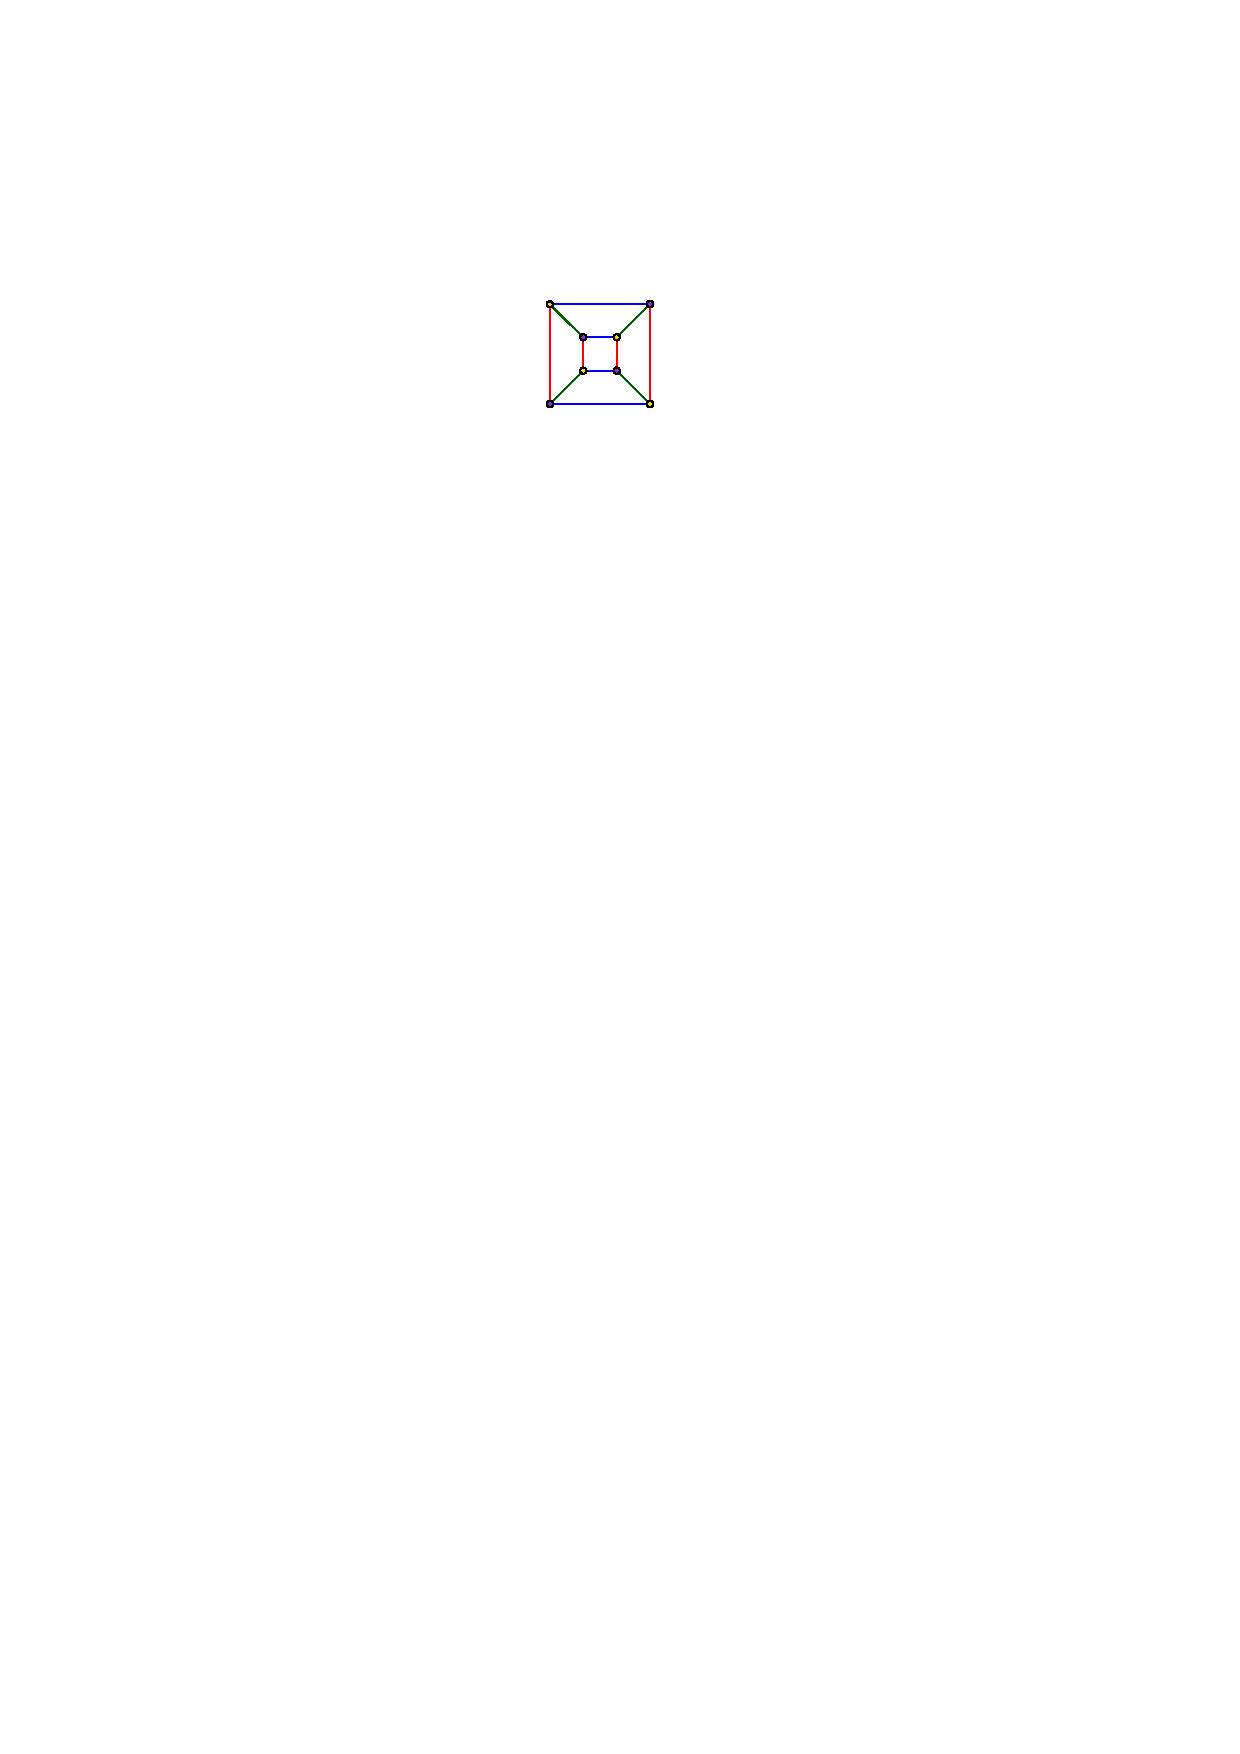
\includegraphics[width=0.2\textwidth]{../Resources/Figs/cubical_tot_colr.pdf}
    \caption{Total coloring of cubical graph using five colors}
    \label{fig:cubical_tot_coloring}
\end{figure}

\begin{figure}[H]
    \centering
    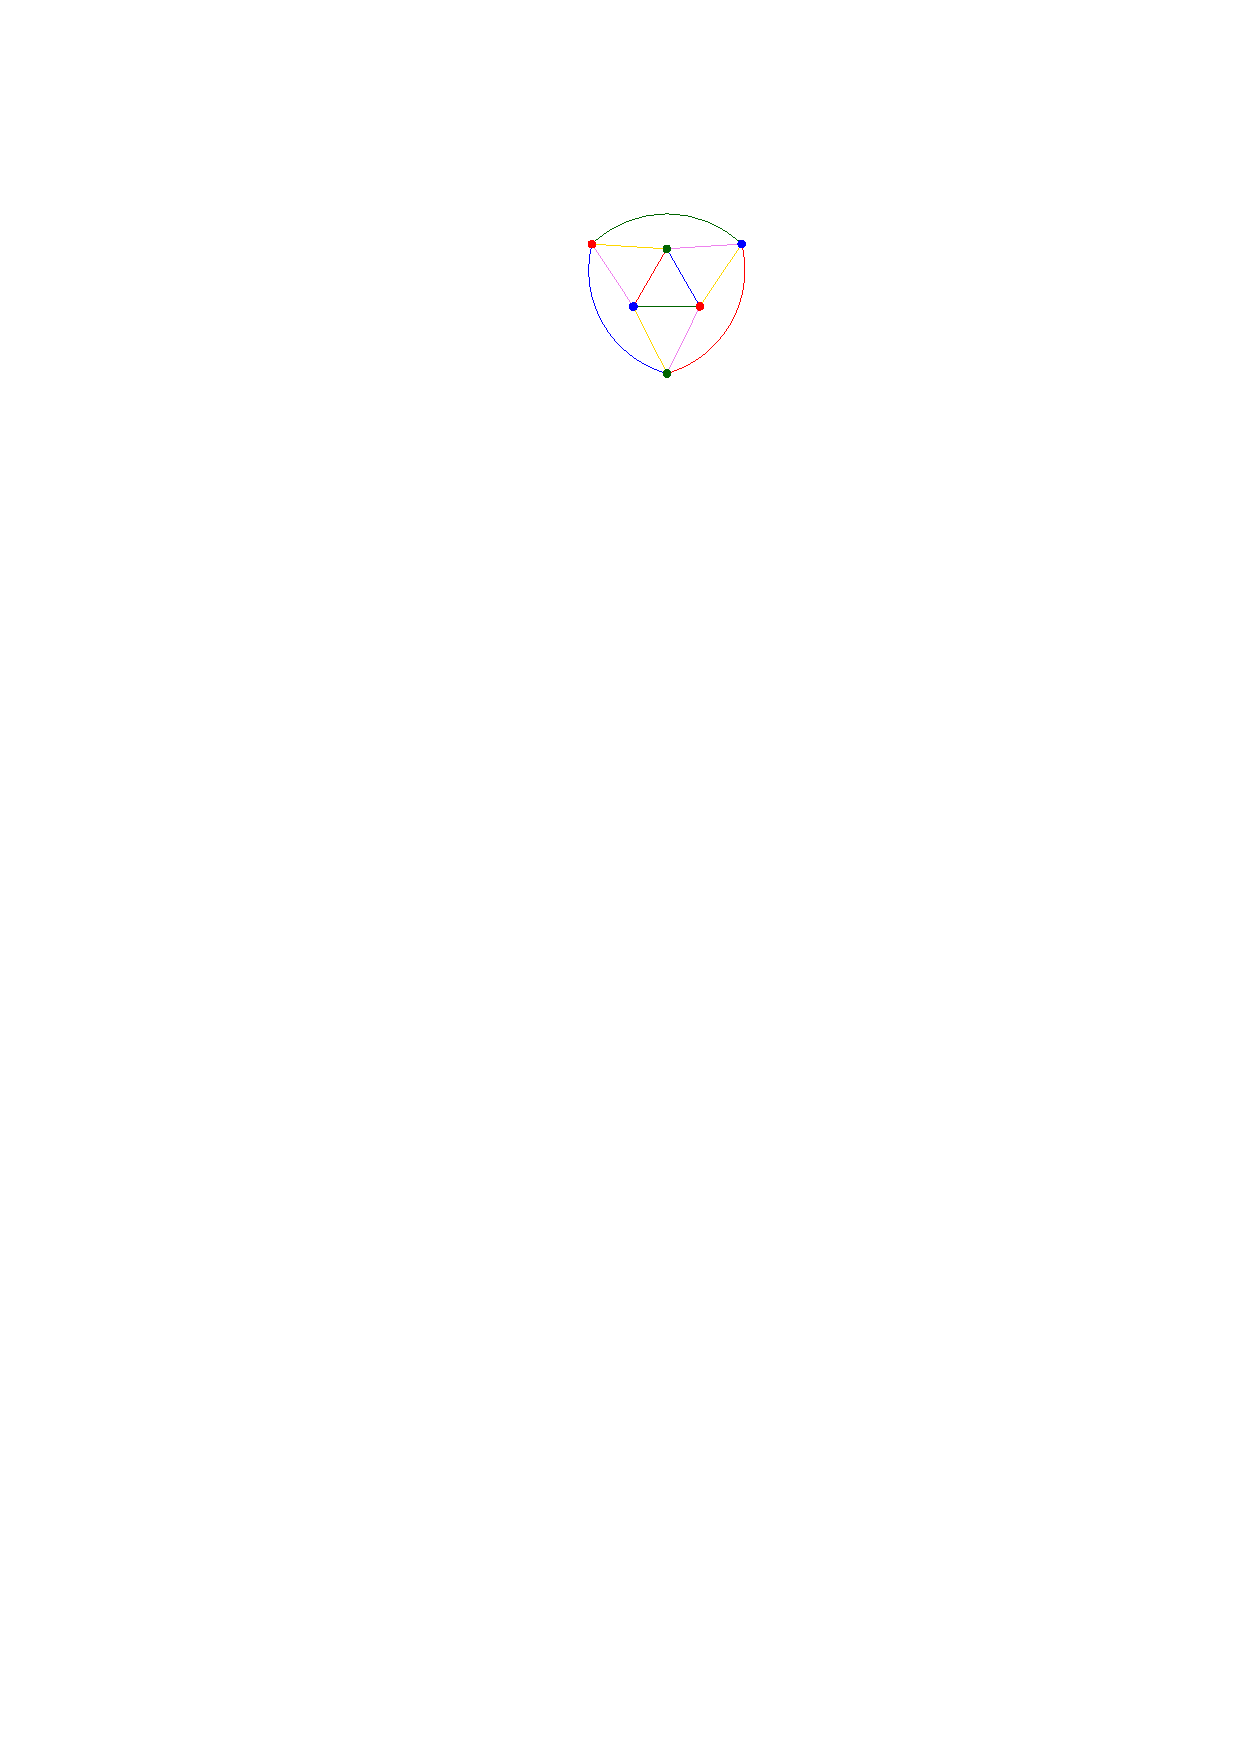
\includegraphics[width=0.2\textwidth]{../Resources/Figs/octahedral_tot_colr.pdf}
    \caption{Total coloring of octahedral graph using five colors}
    \label{fig:octahedral_tot_coloring}
\end{figure}

